\chapter{Drag Torque Constant}\label{app:TorqueTest} 
\textbf{Name: Group 733}\\
\textbf{Date: 04/10 - 2016}

\subsubsection{Purpose}
Finding the relation between the speed of the motor and the drag torque generated by the propeller.

\subsubsection{Setup}
\begin{figure}[H]
	\centering
	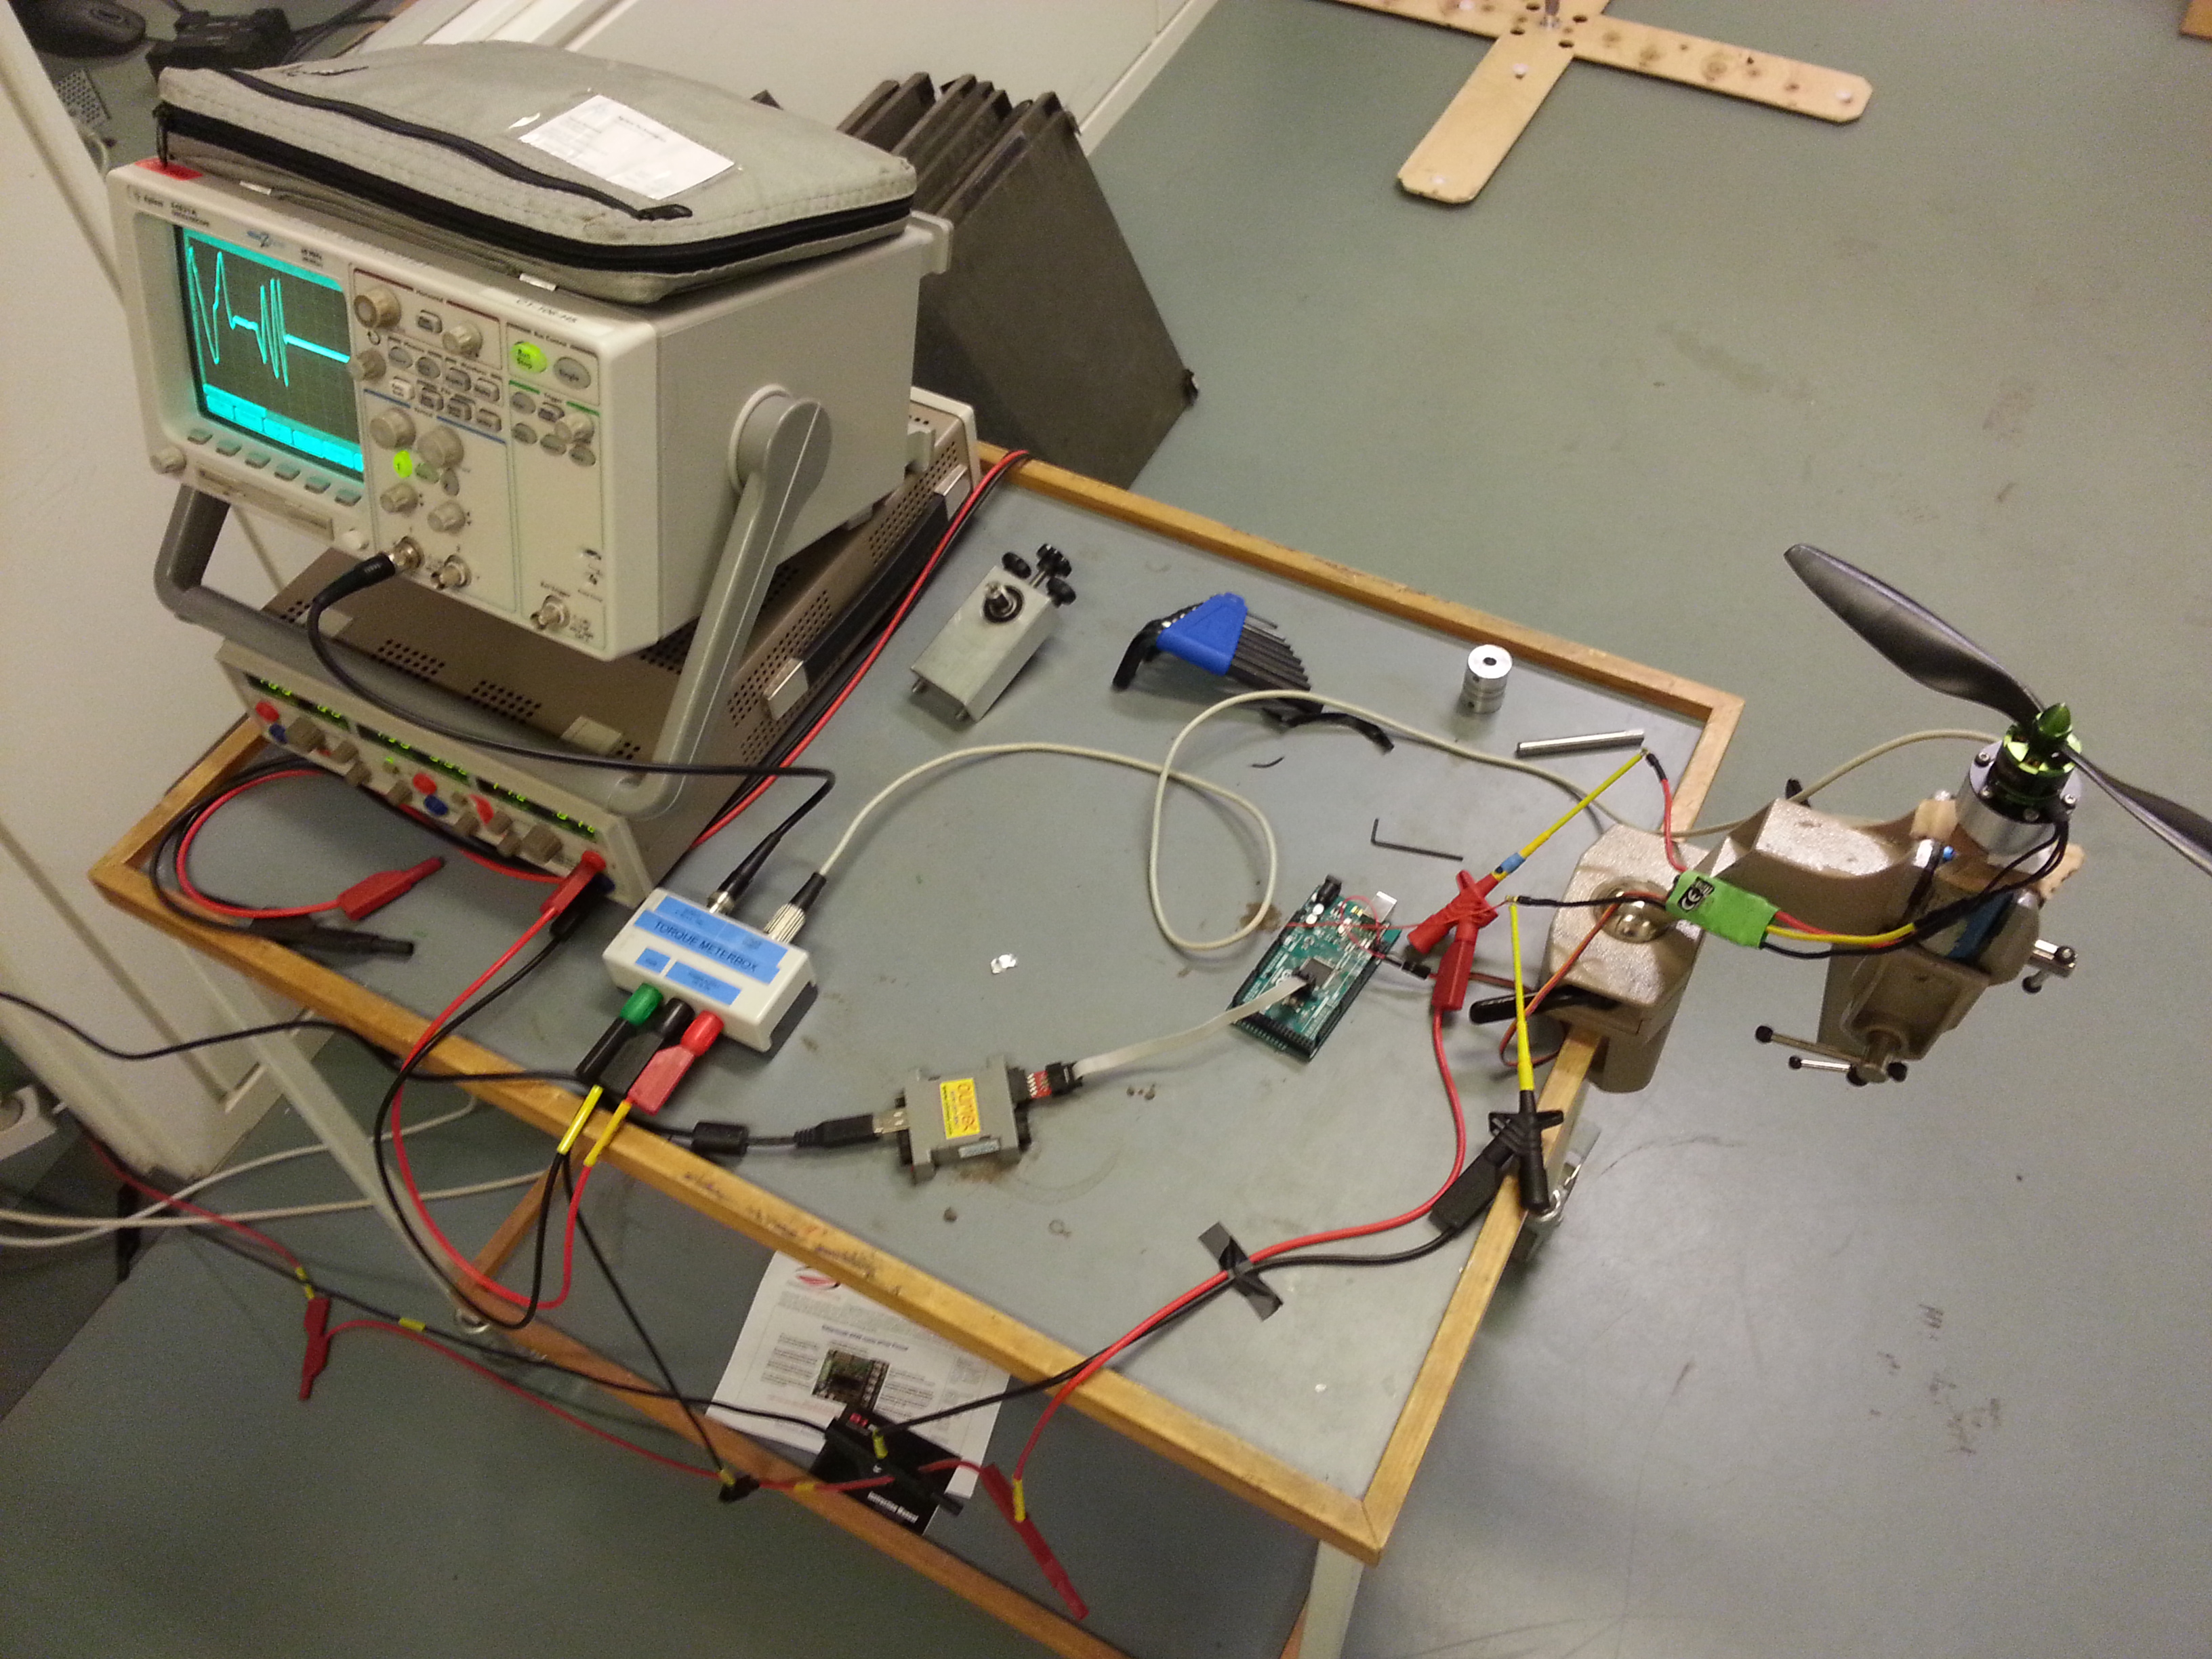
\includegraphics[scale=0.05]{figures/TorqueTestSetup}
	\caption{The setup for the torque test.}
	\label{TorqueTest}
\end{figure}

\subsubsection{List of Equipment}
\begin{table}[H]
	\begin{tabular}{|l|l|p{4.3cm}|}
		\hline%------------------------------------------------------------------------------------------------------------
		\textbf{Instrument}                                  &  \textbf{AAU-no.}  &  \textbf{Type}                       \\
		\hline%------------------------------------------------------------------------------------------------------------
		Tachometer                                           &  08246           &  Shimpo DT-205		                   \\
		\hline%------------------------------------------------------------------------------------------------------------
	    Power Supply (11.1 V) &  64565                   &  ES 030-5                 \\
		\hline%------------------------------------------------------------------------------------------------------------
		Processing Unit                                   &  N/A               & Arduino Mega     \\
		\hline%------------------------------------------------------------------------------------------------------------
		Motor                                         &  N/A               & Multistar 2213-935     \\
		\hline%------------------------------------------------------------------------------------------------------------
		Motor Speed Controller                                   &  N/A               &  -      \\
		\hline%------------------------------------------------------------------------------------------------------------
		Propeller                                   &  N/A               & Turnigy 1045R     \\
		\hline%------------------------------------------------------------------------------------------------------------
		Torquemeter                                   &  N/A               & -     \\
		\hline%------------------------------------------------------------------------------------------------------------
		Oscilloscope                                   & 61604               & Agilent 54621A     \\
		\hline%------------------------------------------------------------------------------------------------------------
		Torquemeter Power Supply                   &  61598              & HM7042-5    \\
		\hline%------------------------------------------------------------------------------------------------------------
		
	\end{tabular}
\end{table}

\subsubsection{Procedure}
\begin{enumerate}
	\item Construct the setup as seen in \figref{TorqueTest}, the power supply is connected to the motor driver and the Arduino Mega is powered from the computer. One PWM pin and GND pin from the board must be connected to the driver signal cables yellow and brown respectively, The torquemeter is connected delivers the measurement as a voltage in the oscilloscope. 
	\item Run the program. It should generate a fixed duty PWM signal in the PWM pin.
	\item Wait for the speed to stabilize and read the torque value as voltage in the oscilloscope. The torque is calculated by considering the the torquemeter specifications. They state that \si{\pm5\textbf{ }V} are equivalent to \si{\pm1\textbf{ }Nm}.
	\item Measure the rotational speed with the tachometer.
\end{enumerate}


\subsubsection{Results}
\begin{table}[H]
	\centering
	\begin{tabular}{|l|l|l|l|p{4.3cm}|}
		\hline%------------------------------------------------------------------------------------------------------------
		\textbf{Motor Speed [rpm]}    & \textbf{Motor Speed [rad/s]} & \textbf{Torque [mV]}  & \textbf{Drag Torque[Nm]} \\ 
		\hline%------------------------------------------------------------------------------------------------------------
		3308 						       &  346.41 				           & 143.8                 & 0.0288         \\
		\hline%------------------------------------------------------------------------------------------------------------
		3416                               &  357.72   			               & 153.1                 & 0.0306         \\
		\hline%------------------------------------------------------------------------------------------------------------
		3655                               &  382.75  			               & 168.8                 & 0.0338         \\
		\hline%------------------------------------------------------------------------------------------------------------
		3755                               &  393.22                           & 171.9                 & 0.0344         \\
		\hline%------------------------------------------------------------------------------------------------------------
		3916 						       &  410.08				           & 206.3                 & 0.0413         \\
		\hline%------------------------------------------------------------------------------------------------------------
		4045                               &  423.59    			           & 212.5                 & 0.0425         \\
		\hline%------------------------------------------------------------------------------------------------------------
		4240                               &  444.02                           & 231.3                 & 0.0463         \\
		\hline%------------------------------------------------------------------------------------------------------------
		4310 						       &  451.34			           & 240.6                 & 0.0481         \\
		\hline%------------------------------------------------------------------------------------------------------------
				
	\end{tabular}
\end{table}
\subsubsection{Results}
The obtained results are shown in \figref{TorqueGraph}. They have been approximated by a parabolic curve by finding a linear relation between the velocity in rad/s squared and the thrust force.

\begin{figure}[H]
	\centering
	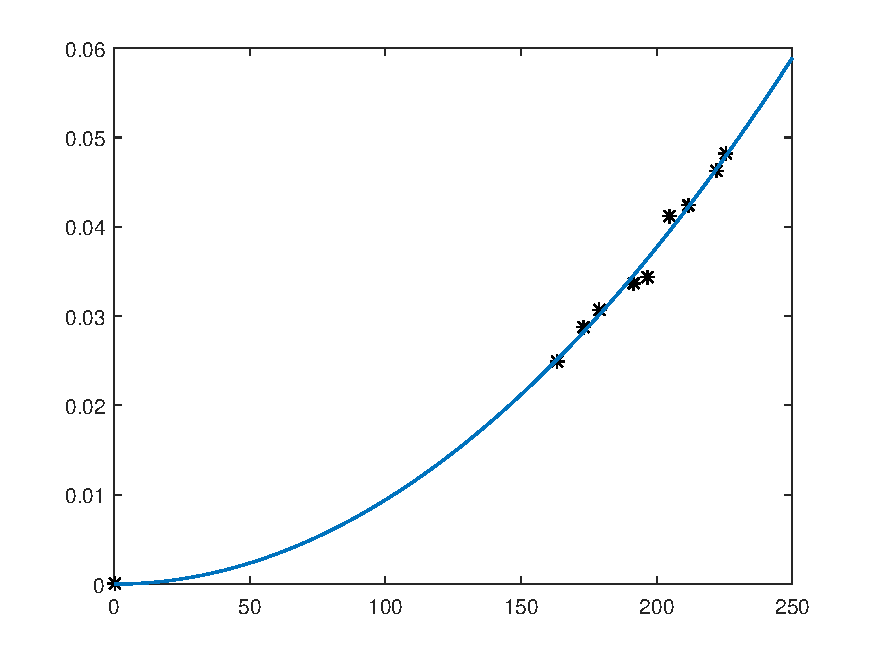
\includegraphics[scale=0.8]{figures/TorqueGraph}
	\caption{Data from the torque test approximated by a parabolic curve.}
	\label{TorqueGraph}
\end{figure}

The resulting constant that provides the relation between the drag torque in the propeller and the velocity squared is $9.39741\cdot10^{-7} Nm\cdot s^2\cdot rad^{-2}$.
